\documentclass[12pt]{report}
\usepackage[left=2cm,right=2cm,
    top=2cm,bottom=2cm,bindingoffset=0cm]{geometry}
\usepackage[russian]{babel}
\usepackage{microtype}
\usepackage{array}
\usepackage{floatflt}
\usepackage{graphicx}
\usepackage{multicol}
\usepackage{caption}
\usepackage{sistyle}
\usepackage{amsmath}
\usepackage{arydshln}
\usepackage{enumerate}
\usepackage{pgfplots}
\usepackage [ warn ] { mathtext }
\usepackage{pgfplotstable}
\usepackage{booktabs}

\usetikzlibrary{circuits}
\usetikzlibrary{circuits.ee}
\usetikzlibrary{circuits.ee.IEC}
\usetikzlibrary{circuits.logic.IEC}
\usetikzlibrary{arrows}
\usetikzlibrary{arrows.spaced} 

\usepackage{fancyhdr}
\usepackage{amssymb}

\pagestyle{fancy}
\fancyhead[L]{ПЛИС}
\fancyhead[R]{2021}

\begin{document}


\section*{\centering \Large Критический путь.}
\indent \indent
Это домашнее задание на одно очко.

Необходимо рассчитать:
\begin{enumerate}
\item
	Критический путь предложенной схемы (рис. \ref{scheme}), считая задержку соединений равной нулю, задержку XOR -- $3t$, задержку AND и OR -- $2t$.
\item
	Пусть входы и выходы схемы подключены к d-flip-flop, задержки в клоках между ними нет (фронт и срез синхросигнала на все триггеры приходит в один и тот же момент), пускай propagation delay каждого триггера равен $t$, setup time $2t$, hold time $3t$. Расчитайте минимально возможный период синхросигнала для такой схемы.
\end{enumerate} 
Обратите внимание, что на схеме есть трех-входовые элементы, их необходимо заменить на эквивалентные схемы из двух-входовых элементов.
В качестве ответа необходимо привести время критического пути, между каким входом и выходом Вы его считали и эквивалентную схему трех-входового элемента.

\begin{figure}[h]
\center{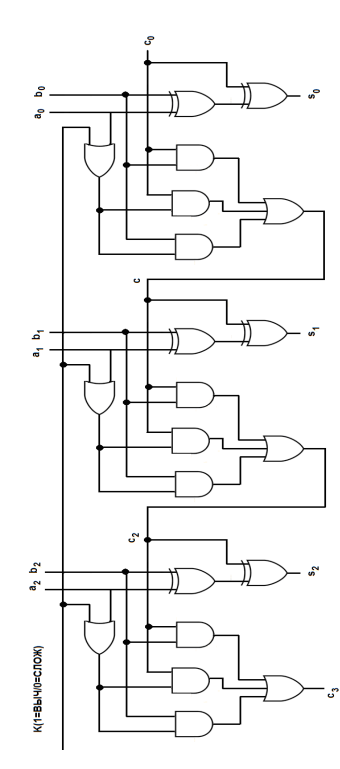
\includegraphics[width=0.35\linewidth]{scheme}}
\caption{Схема 3-х битного сумматора/вычитателя.}
\label{scheme}
\end{figure}




\end{document}